\chapter{BayesQuant: Probabilistic estimation of protein ratios}
\label{chap:model}

\section*{Summary}

The current label-free quantification methods, reviewed in section \ref{sec:quantification} all rely on frequentist statistics, which return point estimates of model parameters such as the estimate of the abundance ratio (fold change) across conditions. However, a Bayesian based approach to this problem, that we know of, is lacking in the literature. As a response to this shortcoming, a statistical model implemented in the probabilistic programming framework Pymc3 was developed and tested on the same benchmark dataset from chapter \ref{chap:pipeline}). The execution of the three steps required when doing Bayesian modelling, mainly (I) model implementation, (II) computation of posterior probabilities and (III) model checking, will be described for this particular problem in the present chapter, together with a discussion on its usability and its strengths.

\section{Introduction}

\subsection{Frequentist and Bayesian statistics}

Both the LFQ and MSqRob quantitication engines presented in chapter \ref{chap:pipeline} took a frequentist approach to the problem of protein quantification. Such approaches, establish a null hypothesis, complementary to the actual hypothesis being tested (alternative hypothesis). The information about the phenomena being modelled is put to use to measure how likely this null hypothesis is via Null-Hypothesis Significance Testing (\ac{NHST}).


\begin{align}
H_0: & \log_2(FC) = 0 \nonumber \\
H_1: & \log_2(FC) \neq 0 \nonumber
\end{align}

The results of this analysis will depend not only of the observed data, but also the data generation process \cite{Kruschke}. This way, both tools returned point estimates of the log2FC between a pair of conditions and a p-value, which provides a measurement of the probability of the null hypothesis. The null hypothesis usually states that the true value of the parameter is 0. Thus, p-values do not say anything about probability of the alternative (our) hypothesis.

The Bayesian statistical framework provides an alternative point of view by revolving the role played by the model parameters and the observed data. While frequentist statistics treats the data as random and the parameters as fixed, a Bayesian framework swaps their roles and yields a probability distribution for any model parameter given the provided data. Bayesian analyses rely on the observed data and prior knowledge about the phenomenon only, and comes equipped with an equation that mathematically formalizes how to introduce these two dependencies in a valid way. This is the so called Bayes\textquotesingle s theorem.

\begin{equation}
P(\theta | y) = \cfrac{P(y | \theta) P(\theta)}{P(y)}
\end{equation}

The Bayes theorem is an extremely versatile tool taking a role analogous to that of statistics like T, F, or $\chi^2$. Unlike them, which are tailored to specific scenarios, it can be used compute the probability distribution of almost any parameter in any model. 4 terms can be distinguished in its expression

\begin{enumerate}

\item $P(\theta)$: the \textbf{prior} probability distribution of the model parameter, introduces previous knowledge about the phenomenon being modelled.

\item $P(y | \theta)$: the probability distribution of the observed data (y) over the possible parameter space. It is also known as \textbf{likelihood} of the model, and its duty is updating our beliefs about the phenomenon by capturing the information in the data.

\item $P(y)$: the probability of the data, defined as the marginal probability of the data given a parameter value, for all possible values. It acts as a normalizing constant that makes the resulting distribution a true probability distribution adding up to 1. It is also known as the data \textbf{evidence}.

\item $P(\theta | y)$: the updated probability distribution of the model parameter, with the information extracted from the observed data. Since it reflects the beliefs about the phenomena after observing data, it is called \textbf{posterior} probability distribution,as opposite to the prior.

\end{enumerate}


The Bayes\textquotesingle s theorem formulated above is thus read as \textit{the posterir probability of the parameter $\theta$ is equal to the \textbf{prior} probability distribution times the likelihood divided by a constant}

It can be applied to the quantification problem, where $\theta$ turns into the log2FC parameter we try to estimate. All is needed is the computation of the posterior probability distribution. Unfortunately, this is tractable analytically for simple models only. However, Markov Chain-Monte Carlo (\ac{MCMC}) methods can be used to approximate this posterior, and are guaranteed to reach an infinitely exact fit if ran for long enough. Their demanding computational cost has only been recently met by the power of modern computers, thus making the approach feasible. Several Bayesian statistics frameworks are available on popular programming languages like R (JAGS) and Python (Pymc3 \cite{Salvatier2016}), all making use of a programming paradigm called \textbf{probabilistic programming}.

\subsection{Probabilistic programming}

The management of uncertainty in statistics is done by means of probability distributions, which account for the possible values that a parameter could take, together with how likely they are. Probabilistic programming offers the framework to build complex statistical models by storing probability distributions as variables of the program. Moreover, probabilistic programming packages supply the tools needed to perform inference with these models by taking experimental evidence (data) and fitting the distributions to the data using Bayes theorem. The fit of the model to the data entails the computation of the posterior probability distribution, which is tallied using \ac{MCMC} algorithms provided with the probabilistic programming tool.

Pymc3 is a mature Python module dedicated to support probabilistic programming. It features   intuitive model specification syntax, modern and powerful \ac{MCMC} sampling algorithms like the No-U-Turn-Sampler (\ac{NUTS}) as well as Automatic Differentiation Variational Inference (\ac{ADVI}) \footnote{\href{https://github.com/pymc-devs/pymc3}{https://github.com/pymc-devs/pymc3}}. Therefore, it provides the tools required to build a Bayesian model for the probabilisitc estimation of protein \ac{log2FC} in proteomics datasets, that is, together with an estimate of its uncertainty.

\subsection{Goals}

\begin{enumerate}

\item Develop a Bayesian model to estimate log2FC in proteomics datasets together with the uncertainty of the estimate.

\item Make it scalable and fast for usability in ordinary modern computers.

\end{enumerate}

\section{Materials and Methods}

\subsection{Data input}
The peptides.txt and proteinGroups.txt files produced by MaxQuant \cite{Cox2008} after the analysis of the dataset published in \cite{Cox2014} were used as input for the modelling algorithm when running without sequence modelling, and processed using the \texttt{preprocess\_MaxQuant} and \texttt{MSnSet2protdata} functions in the MSqRob \cite{Goeminne2016} package, similar to what was done in section \ref{subsec:database_preparation}.

\subsection{Sequence modelling}

When running with active sequence modelling, the peptide sequences and their neighborhood in the protein was extracted from \textit{E. coli} and \textit{Homo sapiens} proteome databases (\ref{subsec:database_preparation}). The protein neighborhood was defined by a window spanning 15 aminoacids on both sides of the peptide. It was extracted using the seqinr \cite{Charif2007} and GenomicRanges \cite{Lawrence2013} packages implemented in R and Bioconductor.

Features to model the peptide effect based on sequence were extracted using BLABLA

\subsection{Bayesian modelling using Pymc3}

In order to get started with Pymc3, we first need to import it.

\begin{minted}[mathescape,
               linenos,
               numbersep=5pt,
               autogobble=true,
               %frame=lines,
               framesep=2mm]{python}


import pymc3 as pm              
\end{minted}

The model is initialized as a Python context manager. Within the context manager, the model is implemented by defining prior distributions for the model parameters and establishing the dependency relationships between them.

The code below formalizes the bias in \ac{MS1} intensity measurements due to a random effect in Pymc3 code.

\begin{minted}[mathescape,
               linenos,
               numbersep=5pt,
               obeytabs=true,tabsize=2,
               firstnumber=last,
               framesep=2mm]{python}

with pm.Model() as model:             
         sigma = pm.HalfNormal('sigma', 1)
         mu = pm.Normal('mu', mu=0, sd=sigma)
\end{minted}


Which is equivalent to the following statistical notation:

\begin{align}
\sigma \sim \mathcal{HN}(1)\,.  \\
\mu \sim \mathcal{N}(0,\,\sigma^{2})\,.
\end{align}

and can be read aloud as \textit{the prior probability distribution of the random effect follows a normal distribution with mean 0 and standard deviation $\sigma$. In turn, $\sigma$\textquotesingle s prior probability distribution follows a half normal distribution with standard deviation 1.}

\textit{hola}


\begin{minted}[mathescape,
               linenos,
               numbersep=5pt,
               obeytabs=true,tabsize=2,
               firstnumber=last,
               framesep=2mm]{python}
effect = pm.Normal("pep", mu, sigma, n_elements)  
\end{minted}


\begin{figure}[!h]
\centering
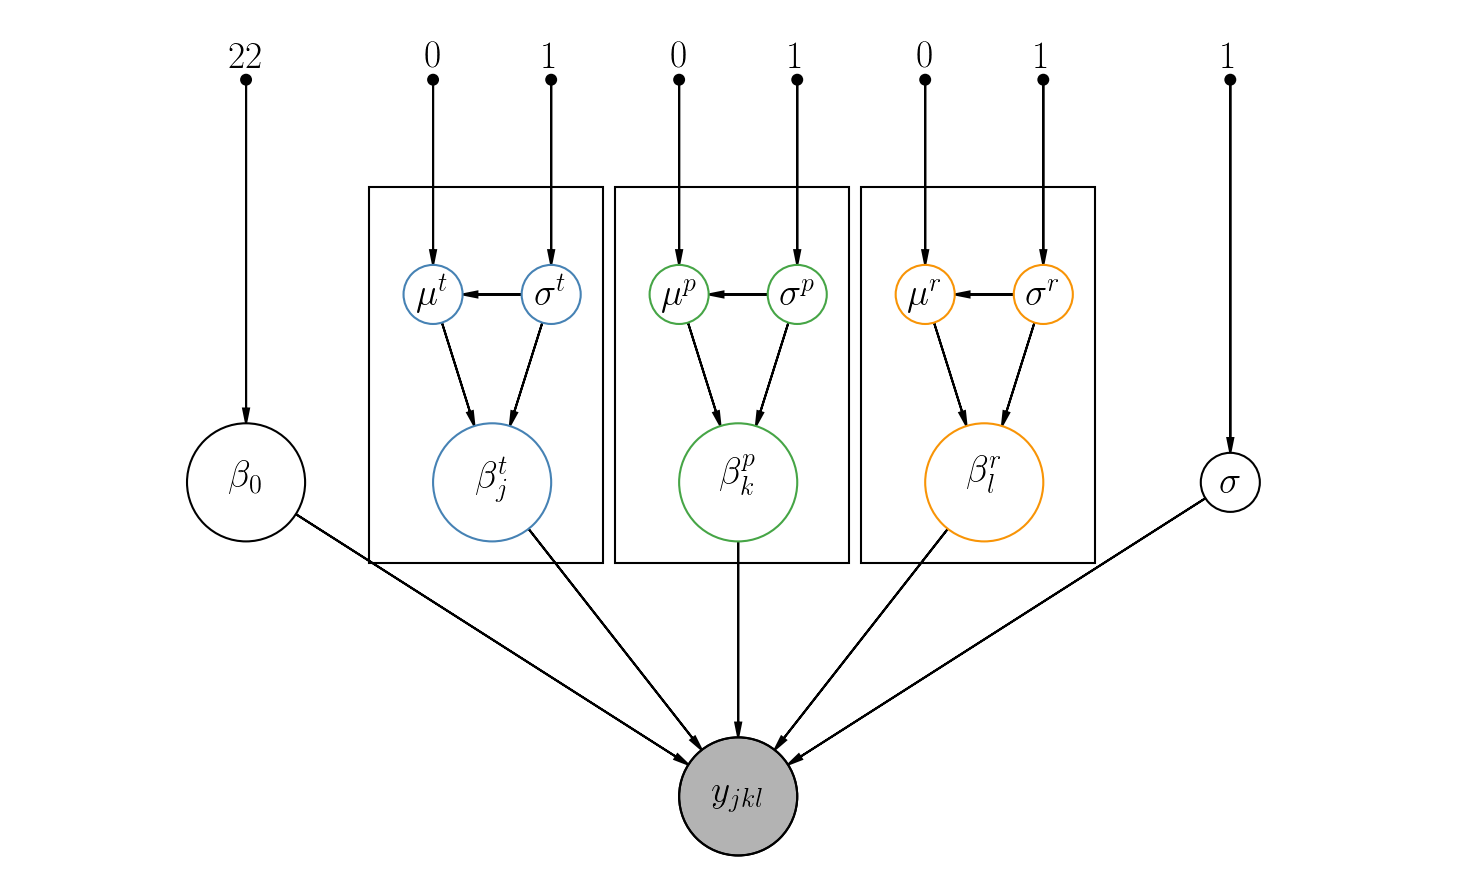
\includegraphics[width=\textwidth]{graph}
\caption{Diagram of the Bayesian model developed in the present paper, without sequence modelling of the peptide effect. It is represented as a Directed Acyclic Graph \ac{DAG} where nodes represent hyperparameters or random variables (in a circle) and directed edges  represent the dependencies between them. The nodes on the top depict the hyperparameters of the model, governing the prior probability distributions represented by the nodes to which their edges lead to. The remaining nodes articulate the probabilistic model and all lead to a final node ($y_{ijkl}$) which represents the modelling of the observed data with the instantiated model.}
\label{fig:daft_model}
\end{figure}



\section{Results}

\subsection{Model implementation (I) peptide as a random process}

\subsection{Model implementation (II) peptide effect with sequence features}

\subsection{Posterior probability distribution computation}

\ac{ADVI} returns good results faster than \ac{NUTS}

\subsection{Model checking}


\section{Discussion}



\section{Conclusion}


%As such, they are the target of multiple regulatory pathways ensuring their quantities are kept within homeostatic ranges.